
\subsection{Funnels}
\label{sec:funnels}

The uncertainty guarantees in this paper is given through creating
\textit{funnels}. Funnels are the parameterization of the \textit{finite time
  reachable sets} for the dynamical system at hand. The following sections will
introduce and develop the theory needed to understand the \ac{SOS} framework
that lies at the bottom of the mathematical verification of these reachable
sets. For the curious reader, a more basic introduction can be found in
Appendix A of my master's thesis at \url[master-thesis]{http://www.github.com/olepor/master-thesis}.

A \textit{funnel} is a parameterization of the reachable set of a dynamical
system. This means that a Funnel holds all the states the dynamical system can
be in during a planning task. Mathematically the reachable set of the system is
defined as
\[
  \vect{x}(0) \in \mathcal{X}_0 \implies \vect{x}(t) \in F(t), \forall t \in
  \sqb{0,T},
\]
where \(\mathcal{X}_0\) is the set of initial conditions, \(\sqb{0,T}\) the time
interval, and \(F(t)\) is the set of states that the system can be in at time
\(t\). Although this paper concerns itself with approximating the reachable set
through \textit{Lyapunov} functions, a useful analogy is imagining the funnel
created through a \textit{Monte-Carlo} simulation, where the funnel is the set
of all the paths traversed by the dynamical system at hand. For the simple
airplane model \cref{eq:model-dynamics}, a Monte-Carlo simulation of nine
starting points along the y-axis, along with a simple \ac{LQR} controller on the
heading of the aircraft, can be seen in \cref{fig:monte-carlo-sim}.

\begin{figure}[!t]
  \centering 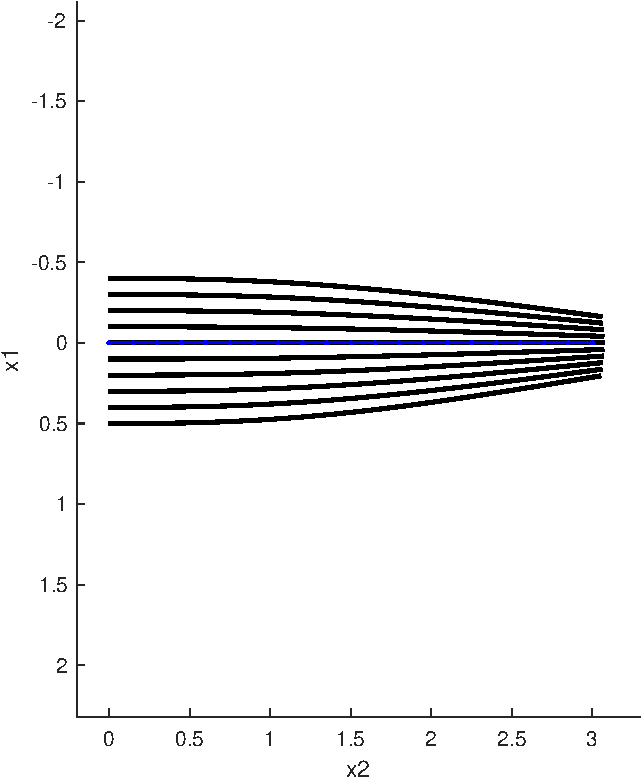
\includegraphics[scale=.6]{figures/preliminaries/montecarlofunnel}
  \caption[Monte-Carlo simulation of the funnel for the \ac{LQR}-controller]{The simulation of N paths starting from a random point in the
    interval \(\sqb{-.5,.5}\), and controlled with a LQR controller.}
  \label{fig:monte-carlo-sim}
\end{figure}

In the literature, the term funnel first appears in
\cite{masonMechanicsManipulation1985}, but is later employed in a lot of
research. The funnel definitions in this thesis is taken from a series of
articles on funnels~\cite{Tobenkin_2011,tedrakeLQRtreesFeedbackMotion2009,
  majumdarRobustOnlineMotion2013,
  majumdarFunnelLibrariesRealtime2017,ahmadi2014dsos}, with the main focus being
on \cite{majumdarFunnelLibrariesRealtime2017}.


\subsection{Computing Funnels}

The funnel computations will be based on the \ac{SOS} theory developed in the
following sections. When given a nominal trajectory, the goal is to compute a
robust invariant set around this trajectory that will guarantee that the planner
is free from collisions during execution of the aforementioned trajectory. This
robustly invariant set is parameterized through Lyapunov function candidates,
that, in this case, will be based upon an \ac{LQR} controller for the system.

In order to compute funnels, a model of the dynamics of the system is required.
Thus, given the nonlinear dynamical system
\begin{equation}
  \dot{\vect{x}} = f\big(\vect{x}(t), \vect{u}(t) \big), \label{eq:dynamicalsystem}
\end{equation}
with \(\vect{x}(t)\) the state of the system at time \(t\), and \(\vect{u}(t)\)
the control input. Assume that an open loop nominal trajectory \(\vect{x}_0
\colon [0,T] \rightarrow \R^n\) with control input \(\vect{u}_0 \colon [0,T]
\rightarrow \R^n\) is given. Where \(\vect{u}_{0}\) is the nominal control
input. Then define a change of coordinates into the error coordinate frame
\begin{align}
  \label{eq:system-error-dynamics}
  \bar{\vect{x}}(t) &= ( \vect{x} - \vect{x}_0 )(t) \\
  \bar{\vect{u}}(t) &= (\vect{u} - \vect{u}_0 )(t) \mathEoS
\end{align}
Then, transforming \cref{eq:dynamicalsystem} to the new coordinate frame one
obtains
\begin{equation}
  \dot{\bar{\vect{x}}} = \dot{\vect{x}} - \dot{\vect{x}}_0 = f\big( \vect{x}_0(t) + \bar{\vect{x}}(t), \vect{u}_0(t) + \bar{\vect{u}}(t) \big) - \dot{\vect{x}}_0(t) \mathEoS \label{eq:dynamicalsystem-coordinatechange}
\end{equation}

In order to compute a parameterized reachable set through \ac{SOS} programming
the system in \cref{eq:dynamicalsystem-coordinatechange} needs to be polynomial,
and hence be parameterized by \(\vect{x}\) and \(t\) polynomially, since the
\ac{SOS} framework can only verify polynomial inequalities. Therefore, through
the use of a \ac{TV-LQR} (although any controller providing a \ac{CLF} can be
used), the control input can be eliminated from the dynamical equation, giving
\begin{equation}
  \label{eq:dynamicclosedloop}
  \dot{\bar{\vect{x}}} = f_{cl}\big( t,\bar{\vect{x}}(t) \big) \mathEoS
\end{equation}
However, the dynamical system may still not be polynomial, which is a necessary
condition in order for the system to be verified using \ac{SOS} programming.
Therefore, by expanding the system in \cref{eq:dynamicclosedloop} around the
nominal trajectory \(\vect{x}_0\), through a Taylor polynomial of some degree
\(N\), the resulting polynomial should be able to capture the nonlinearities of
the system.

The goal is to parameterize a \textit{tight outer approximation} of the set of
states the system may transition into during the time interval \([0,T]\) -- even
in the face of uncertainty. Given that \(F(t)\) is the set of states the
system in \cref{eq:dynamicclosedloop} can be in at time \(t\), then
\begin{equation}
  \label{eq:reachableset}
  \bar{\vect{x}}(0) \in \mathcal{X}_0 \implies \bar{\vect{x}}(t) \in F(t), \, \forall t \in [0,T],
\end{equation}
where \(\mathcal{X}_0\) is the initial condition set, and \(F(t) \subset \R^n\)
is the finite time funnel for the system, is the mathematical description of the
finite time reachable funnel.

\begin{definition}
  \label{def:funnel}
  A funnel associated with a closed-loop dynamical system \(\dot{\bar{\vect{x}}}
  = f_{\mathit{cl}}\big( t,\vect{x}(t) \big) \) is a map \(F \colon [0,T]
  \rightarrow \mathcal{P}(\R^n)\), from the time interval \([0,T]\) to the power
  set (i.e. the set of subsets) of \(\R^n\) so that the sets \(F(t)\) satisfy
  the
  condition in \cref{eq:reachableset}~\cite{majumdarFunnelLibrariesRealtime2017}.
\end{definition}

Next, the reachable set is parameterized through the use of Lyapunov functions,
which yields
\begin{equation}
  F(t) = \set{\bar{\vect{x}}(t) \mid V \big(t, \bar{\vect{x}}(t) \leq \rho (t) \big)},
\end{equation}
where \(\rho (t) \colon [0,T] \rightarrow \R^+\), is an upper bound which limits
the size of the reachable set, and \(V \big(t,\bar{x}(t) \big)\) is a Lyapunov
function \(V \colon [0,T] \times \R^n \rightarrow \R^+\) (in this case a
\ac{CLF}, in the form of a simple \ac{LQR} controller).

Then, by setting \(\mathcal{X}_0 \subset F(0,\bar{\vect{x}})\), one can derive
the sufficient condition~\cref{eq:reachableset} for containing the reachable set
in the Lyapunov function parameterization
\begin{equation}
  \label{eq:funnelsufficient}
  V(t,\bar{\vect{x}}) = \rho(t) \implies \dot{V}(t,\bar{\vect{x}}) < \dot{\rho}(t), \, \forall t \in [0,T], 
\end{equation}
with \(\dot{V}(t,\bar{\vect{x}})\) computed as
\begin{equation}
  \dot{V}(t,\bar{\vect{x}}) = \frac{\partial V(t,\bar{\vect{x}})}{\partial \vect{x}} f_{\mathit{cl}}(t,\bar{\vect{x}}) + \frac{\partial V(t,\bar{\vect{x}})}{\partial t} \mathEoS
\end{equation}

Currently there are no limitations on the functions \(V\) and \(\rho\), and
hence there exists infinitely many functions with different sized reachable sets
that satisfies~\cref{eq:funnelsufficient}, and is a valid funnel in the sense of
~\cref{def:funnel}. Hence, in order for efficient planning to take place, the
motion primitives, meaning the size of the funnels, should be as small as
possible. This is done through minimizing the volume of the funnels using the
following optimization problem

\begin{IEEEeqnarray*}{rCl}
  &\underset{V,\rho}{\text{infimum}} \; &\int_{0}^{T} \vol\big( F(t) \big) \,
  \mathrm{d}t \label{eq:funneloptimizationproblem} \IEEEyesnumber \\
  &\text{subject to} \\
  \IEEEeqnarraymulticol{3}{l}{ V(t,\bar{\vect{x}}) = \rho (t) \implies
    \dot{V}(t,\bar{\vect{x}}) < \rho (t) \, \forall t \in
    [0,T]} \IEEEyessubnumber \label{eq:funnel-optimization-subject-to}   \\
  \IEEEeqnarraymulticol{3}{r}{ \mathcal{X}_0 \subset F(0,\bar{\vect{x}})} \mathEoS \nonumber
\end{IEEEeqnarray} 

\begin{figure}
  % \centering
  % \includegraphics[scale=.7]{figures/experiments/lyapunov_visualization}
  \centering { \fontsize{16pt}{16pt}\selectfont \def\svgwidth{.8\textwidth}
    \import{figures/experiments/}{lyapunov_visualization.pdf_tex} }
  \caption[A converging funnel parameterized through a Lyapunov function]{A visualization of the Lyapunov function along a trajectory, where
    the center of the Lyapunov function moves along the trajectory with time
    \(t\).}
\end{figure}


\subsection{Formulating the Optimization Problem as a SOS Program}

The optimization problem in \eqref{eq:funneloptimizationproblem} would be
impossible to solve efficiently had it not been for advances in mathematical
convex numerical optimization by
\citeauthor{parilloStructuredSemidefinitePrograms}~\cite{parilloStructuredSemidefinitePrograms},
as in general the problem involves searching over an infinite function space.
While the general optimization problem of searching through an infinite function
space is not amenable to efficient numerical computation, the problem can be
made computationally feasible through the use of a \ac{SOS} programming
approach~\cite{tedrakeLQRtreesFeedbackMotion2009}.

Thus in order to make the problem amenable to a \ac{SOS} program, there are a
few requirements that need to be met by the problem formulation. Firstly the
initial condition set needs to be a \textit{semi-algebraic set}, (i.e.
parameterized by polynomial inequalities) so that
%
\begin{equation}
  \label{eq:initial-condition-set-parameterized}
  \mathcal{X}_0 = \set{\bar{\vect{x}} \in \R^n \mid g_{o,i}(\bar{\vect{x}}) \geq 0, \, i = 1,\ldots,N_0},
\end{equation}
%
is the initial condition set. Then rewriting \cref{eq:funnelsufficient} in terms
of positivity and equality constraints yields
\begin{equation}
  V(t,\bar{\vect{x}}) = \rho(t) \implies \dot{\rho}(t) - \dot{V}(t,\bar{\vect{x}}) > 0,
\end{equation}
and the initial condition set \eqref{eq:initial-condition-set-parameterized} is
rewritten
\begin{equation}
  g_{0,i}(\bar{\vect{x}}) \geq 0 \, \forall i \in \set{1,\ldots,N_0} \implies \rho(0) - V(0,\bar{\vect{x}}) \geq 0 \mathEoS
\end{equation}
Which, if these functions are both polynomial, is now in the form of a \ac{SOS}
optimization problem. Then through the use of the \nameref{sec:s-procedure} one
can write the optimization problem~\eqref{eq:funneloptimizationproblem} as
\begin{IEEEeqnarray*}{rl}
  \dot{\rho}(t) - \dot{V}(t,\bar{\vect{x}}) - L(t,\bar{\vect{x}}) \big(
  V(t,\bar{\vect{x}}) - \rho(t) \big)& \nonumber
  \\
  - L_{t}(t,\bar{\vect{x}})\big( t\left( T - t \right) \big)& \, \text{is
    SOS} \IEEEeqnarraynumspace \IEEEyesnumber \label{eq:sufficient-conditions} \\
  \rho(0) - V(0,\bar{\vect{x}}) - \sum_{i}^{N_{0}}
  L_{0,i}(\bar{\vect{x}})g_{0,i}(\bar{\vect{x}}) & \, \text{is
    SOS} \IEEEyessubnumber \label{eq:sufficient-conditions-2} \\
  L(t, \bar{\vect{x}}), \, L_{t}(\bar{\vect{x}}), \, L_{0,i}(\bar{\vect{x}})& \, \text{are SOS}, \nonumber
  \\
  \IEEEeqnarraymulticol{2}{r}{\forall i \in \set{1,\ldots,N_{0}}}, \nonumber
\end{IEEEeqnarray*}
where \(L\), \(L_{t}\), and \(L_{0,i}\) are multiplier polynomials~(see
\cref{sec:s-procedure}).

The goal is to make the parameterization of the reachable set as small as
possible, and therefore minimizing the cost function in
\eqref{eq:funneloptimizationproblem}. This is done by \cite{Tobenkin_2011}
through approximating the cost function by first discretizing the problem and
replacing the integral with a finite sum
\begin{equation}
  \int_{0}^{T} \vol\big( F(t) \big) \, \mathrm{d}t \rightarrow \sum_{k=1}^{N} \vol\big( F(t_{k}) \big) \mathEoS \label{eq:discrete-costfunction}
\end{equation}
Since the Lyapunov function \(V(t,\bar{\vect{x}})\) in this paper is quadratic,
it can be written as
\begin{equation}
  V(t_{k}, \bar{\vect{x}}) = {\bar{\vect{x}}}^{T}S_{k}\bar{\vect{x}}, \, S_{k} \succeq 0,
\end{equation}
where \(\succeq 0\) means that the matrix is positive semi-definite. Since the
set \(F(t_{k})\) is now an ellipsoid in which the volume can be minimized
through maximizing the determinant of \(S_{k}\), which in turn can be
transformed into a \acl{SDP} problem. If an upper bound
on the cost function \cref{eq:discrete-costfunction} is introduced as
\begin{equation}
  \mathcal{E} (t_{k}) = \set{\bar{\vect{x}} \in \R^n \mid {\bar{\vect{x}}}^{T}S_{k}\bar{\vect{x}} \leq 1, \, S_{k} \succeq 0},
\end{equation}
where \( \mathcal{E} ( t_{k} ) \) is an ellipsoid containing the reachable set
\( F ( t_{k} ) \) at time \( t_{k} \). Then this containment constraint can be
equivalently expressed as
\begin{equation}
  V ( t_{k}, \bar{\vect{x}} ) \leq \rho(t_{k})  \implies {\bar{\vect{x}}}^{T}\matr{S}_{k}\bar{\vect{x}} \leq 1 \mathEoS
  \label{eq:discrete-containment-constraint}
\end{equation}
Which when expressed using \ac{SOS} constraints gives
\begin{align}
  1 - {\bar{\vect{x}}}^{T}\matr{S}_{k}\bar{\vect{x}} - L_{\mathcal{E},k}(\bar{\vect{x}}) \big( \rho(t_{k}) - V(t_{k}, \bar{\vect{x}}) \big)  \qquad \text{is SOS}& \\
  L_{\mathcal{E},k}(\bar{\vect{x}}) \qquad \text{is SOS}& \mathEoS \nonumber
\end{align}
%
Then combining the cost function~\eqref{eq:discrete-costfunction} with the
constraints in Equation~\eqref{eq:discrete-containment-constraint} along with
\eqref{eq:sufficient-conditions}\eqref{eq:sufficient-conditions-2}, one arrives at the
following optimization problem:
  \newcommand{\E}{\mathcal{E}}
  \begin{mini!}[3]
    { \substack { V, \rho, L, L_t,
        \\
        L_{0, i}, S_{k}, L_{\E, k} } }
    { \sum_{k = 1}^{N} \vol \bigl( \E(t_{k}) \bigr) = \nonumber}
    {\label{opt:time-dependent-optimization-problem}}
    {}
    \breakObjective{\sum_{k = 1}^{N} \vol \bigl( \set{\vect{x} \mid \vect{x}^{T} \matr{S}_{k} \vect{x}
        \le 1} \bigr) }
    \addConstraint {
        \dot{\rho}(t) -
      \dot{V}(t,\vect{x}) - L(t,\vect{x}) \bigl( { V(t,\vect{x}) - \rho(t) }
      \bigr) \nonumber }
    {}
    {}
    \addConstraint{- L_t (t,\vect{x}) \bigl(  {t \p*{T - t}} \bigr) }
    {}
    {\text{ is SOS}}
    \addConstraint {\rho(0) - V(0, \vect{x}) - \sum_i^{N} L_{0,
        i}(\vect{x}) g_{0, i}(\vect{x}) }
    {}%
    {\text{ is SOS}}
    \addConstraint { 1 - \vect{x}^T \matr{S}_k \vect{x} -
      L_{\E, k}(\vect{x}) \bigl(  {\rho(t_k) - V(t_k, \vect{x})} \bigr) }
    {}%
    {\text{ is SOS}}
    \addConstraint {S_k \nonumber}%
    {\succeq 0}%
    {\forall k \in \set{1, \ldots, N}}
    \addConstraint {L(t,\vect{x}), L_t (t, \vect{x}),\, L_{0,i}(\vect{x}),\,
      L_{\mathcal{E},k}(\vect{x}) \nonumber }%
    {\text{ are SOS}}%
    {\forall i \in \set{1, \ldots, N_0},}
    \addConstraint{\nonumber}
    {}
    {\forall k \in \set{1, \ldots, N} \mathEoS }
  \end{mini!}
This is the continuous finite dimensional optimization problem that is needed in
order to search for a Lyapunov function candidate that parameterizes the
reachable set for the dynamical system at hand.

However, this optimization problem is not in general convex, as the first
constraints are \textit{bilinear} in the decision variables, since \(L\) and
\(V\) are multiplied together. However, the problem can be solved, although not
optimally, if \(V\) and \(\rho\) are held fixed, while the other decision
variables are free. Likewise, fixing \(L\) and \(L_{\mathcal{E},k}\), creates
another \ac{SOS} optimization program. Therefore shifting between the two sets
of decision variables \(\left( L,L_{t},L_{0,i},L_{\mathcal{E},k} \right) \) and
\(\left( V,\rho,L_{0,i},\matr{S}_{k} \right) \)
\textcite{majumdarFunnelLibrariesRealtime2017} arrives at
\cref{alg:funnelalgorithm} on page~\pageref{alg:funnelalgorithm} for computing
funnels.

\begin{figure}[!t]
  \caption{Funnel computation}
  \label{alg:funnelalgorithm}
  \begin{algorithmic}[0]
    \Procedure{FunnelComputation}{\(V,\rho\)}
    \State Output: Funnel
    \State \(\mathnormal{cost}_{\mathnormal{prev}} = \infty\)
    \State converged = false
    \While {\( \neg \mathnormal{converged}\)}
    \State Optimization Problem 1:
    \State %
    \begin{align*}
      \underset{\substack{L,L_{t},L_{0,i},S_{k},L_{}}}{\inf}&  \sum_{k=1}^{N} \vol \bigl( \mathcal{E}(t_{k}) \bigr) & \\    
      \text{subject to } & V \text{ and } \rho \text{ constant.}& \\
    \end{align*}
    \State Optimization Problem 2:
    \State %
    \begin{align*}
      \underset{\substack{V,\rho, L_{t},L_{0,i},S_{k}}}{\inf}&  \sum_{k=1}^{N} \vol \bigl( \mathcal{E}(t_{k}) \bigr) & \\    
      \text{subject to } & L \text{ and } L_{\mathcal{E},k} \text{ constant.}& \\
    \end{align*}
    \State cost = \(\sum_{k=1}^{N} \vol \bigl( \mathcal{E}(t_{k}) \bigr) \)
    \State
    \If{\(\frac{\mathrm{cost}_{\mathit{prev}} -
    \mathrm{cost}}{\mathrm{cost}_{\mathit{prev}}} < \epsilon \) }
    \State converged = true
    \EndIf
    \State \(\mathrm{cost}_{\mathit{prev}} = \mathrm{cost}\)
    \EndWhile
    \EndProcedure
  \end{algorithmic}
\end{figure} 


\subsection{Approximation via Time-Sampling}

It is often the case that the nominal trajectory \(x_{0} \colon [0,T]
\rightarrow \R^n\) is difficult to approximate with a low degree polynomial in
time~\cite{majumdarFunnelLibrariesRealtime2017}. This can cause funnel
computation to take a lot of time, therefore approximating the polynomial
discretely speeds up the calculation, at the cost of exactness. However the
resulting funnels are shown to be acceptable approximations, where exactness can
be regained through increasing the sampling rate~\cite{Tobenkin_2011}. If
\(t_{k} \in [0,T]\), where \(k \in \set{1,\ldots,N}\), the optimization
\cref{opt:time-dependent-optimization-problem} becomes:
\begin{mini!}[3]
  {\substack{V_{k}, \rho, L_{k},\\ L_{0,i}, S_{k},
      L_{\mathcal{E},k}} } % Optimization variables
  {\sum_{k=1}^{N}\vol(\mathcal{E} \bigl(t_{k}) \bigr)} % Optimization function
  {\label{opt:discrete}} % Label optimization problem
  {} % Optimization result
  \breakObjective{= \sum_{k=1}^{N} \vol\left(
    \set{\bar{x} \mid {\bar{x}}^{T} S_{k} \bar{x} \leq 1}
    \right)}
  % Constraints
  %
  %
  \addConstraint{\dot{\rho}(t_{k}) - \dot{V}_{k}(\bar{\vect{x}}) -
    L_{k}(\bar{\vect{x}}) \bigl( V_{k}(\bar{\vect{x}}) - \rho(t_{k}) \bigr)}
                {}
                {}
                \addConstraint{}
                              {}
                              {\forall k \in \set{1,\ldots,N}}
                %
                %
                %
                \addConstraint{\rho(t_{1}) -
    V_{1}(\bar{\vect{x}}) - \sum_{i}^{N_{0}} L_{0,i}g_{0,i}(\bar{\vect{x}})}
  {}
  {\, \text{is SOS}}
  %
  %
  %
  \addConstraint{1 - {\bar{\vect{x}}}^{T} S_{k} \bar{\vect{x}} -
    L_{\mathcal{E},k} \bigl( \rho(t_{k}) - V_{k}(\bar{\vect{x}}) \bigr) }
  {}
  {\, \text{is SOS},}
  \addConstraint{}
  {}
  {\forall k \in \set{1,\ldots,N} \nonumber} %
  %
  %
  %
  \addConstraint{S_{k} \succeq 0}
  {}
  {\forall k \in \set{1,\ldots,N} \nonumber} %
  %
  %
  %
  \addConstraint{L_k(\bar{\vect{x}}),\,L_{0,i}(\bar{\vect{x}}),
    L_{\mathcal{E},k}}
  {\qquad \text{are SOS} \nonumber}
  {\forall i \in \set{1,\ldots,N_0} , \nonumber} %
  %
  %
  %
  \addConstraint{}
  {}
  {\forall k \in \set{1,\ldots,N} \mathEoS \nonumber}
\end{mini!}
This is the same optimization problem as in
\cref{opt:time-dependent-optimization-problem}, but with the continuous time
dependency removed from the equations. This leads to vastly greater performance
in computing the funnels, but the parameterization of the funnels will be
slightly larger, as exactness is lost~\cite{Tobenkin_2011}.


\subsection{Funnel Composition}

Now that discrete motion primitives in the form of funnels can be calculated for
a given base set of trajectories, it is time to handle the overarching goal of
creating a plan consisting of multiple funnels stacked from start to finish, so
that safe traversal can be guaranteed along the given path. In order for two
funnels to create one extended motion primitive from multiple smaller
primitives, the funnels in use must be composable. In order for two funnels to
be composable, the outlet of one funnel needs to be completely contained within
the inlet of the other. This means that if \(\mathcal{F}_1 = F_1(T)\) is the
outlet of funnel \(F_1\), and \(\mathcal{F}_2 = F_2(0)\) is the inlet of
\(F_2\), then
\begin{equation}
  \label{eq:funnel-subset}
  \mathcal{F}_1 \subseteq \mathcal{F}_2
\end{equation}
is required in order for the funnels to be composable.
\begin{definition}
  \label{def:funnel-composition}
  An ordered pair \((F_{1}, F_{2})\) of funnels \(F_1 \colon [0,T_1] \rightarrow
  \mathcal{P}(\R^n)\) and \(F_2 \colon [0,T_2] \rightarrow \mathcal{P}(\R^n)\)
  are sequentially composable if \(F_1(T) \subseteq F_2(0)\).
\end{definition}
Because the implication
\begin{equation}
  V_1(T_1,\bar{\vect{x}}) \leq \rho_1(T_1) \implies V_2(0,\bar{\vect{x}}) \leq
  \rho_2(0)
\end{equation}
is an equivalent condition to \cref{eq:funnel-subset}, and because it can be
checked through the following \ac{SOS} program
\begin{IEEEeqnarray*}{lC}
  \text{Find } \; L(\bar{x}) \IEEEyesnumber \\
  \text{s.t.} \\
  \IEEEeqnarraymulticol{2}{l}{\rho_2(0) - V_2( 0,\bar{\vect{x}}) - L(\bar{\vect{x}})
                  \bigl( \rho_1(T_1) - V_1(T_1,\bar{\vect{x}}) \bigr) \quad \text{is SOS}} \mathEoS \nonumber
\end{IEEEeqnarray*}
Hence funnel composition can be checked in the same way that the funnels are
generated -- through a \ac{SOS} program. Also note that the above program is a
simple search for existence, and hence no cost function is needed.

However in
\citeauthor{majumdarFunnelLibrariesRealtime2017}~\cite{majumdarFunnelLibrariesRealtime2017},
the program is stated simply, and it can be helpful to take a look at the
derivation in order to gain a feel for the implementation of a \ac{SOS} program.

The \nameref{sec:s-procedure} enables the search to be limited to a
semi-algebraic set. In this case, that set is \(\mathcal{F}_2 = \set{\vect{x}
  \in \R^n \mid V_2(0,\bar{\vect{x}}) \leq \rho_2(0)}\), and any \(\vect{x}\)
that is not in this set is therefore not of importance. In more general terms
this can be written
\begin{equation}
  \label{eq:example-s-procedure-implication}
  \vect{x} \in \mathcal{F}_2 \implies p(\vect{x}) \geq 0,
\end{equation}
where \(p(\vect{x})\) is the \ac{SOS} polynomial that is to be verified. In this
case \(p(\vect{x})\) is \(V_2(0,\bar{\vect{x}})\). Thus in order to impose the
implication~\eqref{eq:example-s-procedure-implication} define
\begin{equation}
  q(\vect{x}) = V_2(0,\bar{\vect{x}}) - \rho_2(0) - L(\bar{\vect{x}}) \bigl(
    \rho_1(T_1) - V_1(T_1,\bar{\vect{x}}) \bigr),
\end{equation}
where \(q(\vect{x})\) and \(L(\bar{\vect{x}})\) need to be SOS polynomials.

\begin{example}

  As a simple example, look at embedding a square within a circle. Give the
  circle a radius of \(\sqrt{2}+\epsilon\), and the square with sides of \(2\),
  and center them both at the origin in the Euclidean plane. Then define the
  square
  \begin{equation}
    \label{eq:beta-orig}
    \beta = \set{\vect{x} \in \R^2 \mid \norm{\vect{x_{i}}} \leq 1, \, i=1,2},
  \end{equation} 
  using the Manhattan metric. Then the implication
  \begin{equation}
    \vect{x} \in \beta \implies p(\vect{x}) \geq 0,
  \end{equation}
  is needed in order to write this into a \ac{SOS} program through the use of
  the \nameref{sec:s-procedure}. Then \eqref{eq:beta-orig} can be parameterized
  by a positivity constraint
  \begin{align}
    \beta &= \set{\vect{x} \in \R^2 \mid 1 \pm \vect{x} \geq 0 }, \\
    p(\vect{x}) &= r^2 - x^2 - y^2
  \end{align}
  where \(p(\vect{x})\) is the parameterization of the circle, and \(\beta\) is
  the parameterization of the square with sides of length two. What needs to be
  shown is that \(p(x)\) is positive on the set \(\beta\). Through the
  \nameref{sec:s-procedure} this can be written as the search for a nonnegative
  polynomial \(L_{\mathit{\mathit{ineq}},i}(\vect{x})\) such that \(p(\vect{x}) \geq
  L_{\mathit{\mathit{ineq}},i}(\vect{x})g(\vect{x}) \). Thus
  \begin{equation}
    q(\vect{x}) = p(\vect{x}) -
    \sum_{i=1}^{2}L_{\mathit{\mathit{ineq}},i}(\vect{x})g_{\mathit{\mathit{ineq}},i}(\vect{x}) \geq 0 \forall x \in \beta,
  \end{equation} 
  is required for \(q(\vect{x})\) to be a \ac{SOS} polynomial. From this it is
  seen that when a point satisfies \(g_{\mathit{\mathit{ineq}},i}\) (i.e., when
  \(\vect{x} \in \beta\)) the term \( -
  \sum_{i=1}^{2}L_{\mathit{\mathit{ineq}},i}(\vect{x})g_{\mathit{\mathit{ineq}},i}(\vect{x})\)
  is negative, and hence \(p(x)\) must be nonnegative for \(q(\vect{x})\) to be
  positive. Meaning that \(x \wedge y\) is less than \(r\) on the set \(\beta\).
  Therefore all the points in \(\beta\) are within the bound of the circle, and
  is what verifies the desired implication.

  Solving this problem can be done using any of a number of \ac{SOS} modeling
  software tools. This example relies on \textsc{Yalmip}~\cite{Lofberg2004} and
  its \ac{SOS} programming functionality for \matlab~\cite{Lofberg2009} .


  \lstinputlisting{figures/funnel/embededsquare.m}

  Which returns ``Composition successful!'' for circles with radii larger than
  \(\sqrt{2}\) as expected.
\end{example}


\subsection{Cyclic Coordinates and Lagrangian Dynamics}
\label{subsec:cyclic-coordinates}

With the ability to create a base set of funnels, and verify their ability to be
composed together to create longer motion primitives, the time has come to move
funnels from the initial base set around the world space of the planning
problem. Thus, in order to move funnels around the world space, the dynamics of
the system must not change along the coordinates at which the system is
manipulated. This can be achieved through the theory of cyclic and non-cyclic
coordinates, stemming from Lagrangian dynamics. Therefore, given the Lagrangian
\(\mathcal{L}(q_i, \dot{q_i}, t)\) of a dynamical system, where the \(q_i\) are
the generalized coordinates of the system, and \(\dot{q_i}\) are the generalized
velocities. If the Lagrangian does not contain the \(q_j\) then \(q_j\) is a
cyclic coordinate of the system, and the j-th Lagrangian has the form
\[
  \left( \frac{d}{dt} \right) \left( \frac{\partial \mathcal{L}}{\partial
      \dot{q_j}} \right) = \mathrm{constant} \mathEoS
\]
This means that any \(q_j\) fulfilling the above criteria can be freely moved
around in the state-space, yet yield the same dynamical solution of the system.


\subsection{S-Procedure}
\label{sec:s-procedure}

The \textit{S-procedure} is used in this thesis to check for positivity for the
polynomial at hand over a region given by the set \(\beta\), where
\[
  \beta = \set{\vect{x} \in \R^n \mid g_{eq,i}(\vect{x}),\,g_{ineq,i}(\vect{x})
    \geq 0} \mathEoS
\]
The interest is in showing that a polynomial \(p(\vect{x})\) is nonnegative on
the given set \(\beta\) \ie
\[
  \vect{x} \in \beta \implies p(\vect{x}) \geq 0,
\]
which can be imposed by the following SOS constraints
\begin{IEEEeqnarray*}{rl}
  q(\vect{x}) &= p(\vect{x}) - \sum_{i=1}^{N_{eq}}L_{eq,i}(\vect{x})g_{eq,i}(\vect{x}) \\ 
  &-\sum_{j=1}^{N_{ineq}}L_{ineq,i}(\vect{x})g_{ineq,j}(\vect{x}) L_{ineq,j}(\vect{x}) \\ 
  \IEEEeqnarraymulticol{2}{r}{\text{ is SOS } \forall j \in \set{3,\ldots,N_{ineq}},}
\end{IEEEeqnarray*} 
where the multiplier polynomials \(L_{eq}\) and \(L_{ineq}\) are similar to
Lagrange multipliers in constrained optimization.
